  

\documentclass{beamer}



\mode<presentation>
{
  \usetheme{Warsaw}


}


\usepackage[english]{babel}
% or whatever

\usepackage[utf8]{inputenc}
% or whatever

\usepackage{times}
\usepackage[T1]{fontenc}
% Or whatever. Note that the encoding and the font should match. If T1
% does not look nice, try deleting the line with the fontenc.

\usepackage{amsthm}
\usepackage{amssymb}
\usepackage{amsmath}

\usepackage[nodisplayskipstretch]{setspace}
\setstretch{.2}

\newtheorem{proposition}{Proposition}
\newtheorem{conjecture}{Conjecture}
\newtheorem{ourproblem}{Our Problem}
\newtheorem*{definition*}{Definition}


\title
{Construction of Families of Permutation Trinomials over Finite Fields}

\author
{Christian A. Rodriguez\\
Alex D. Santos}

\institute[]
{
  Department of Computer Science\\
  University of Puerto Rico, R\'{i}o Piedras
}

\date
{\today}



% If you wish to uncover everything in a step-wise fashion, uncomment
% the following command: 

%\beamerdefaultoverlayspecification{<+->}

\begin{document}

\begin{frame}
  \titlepage
\end{frame}

\begin{frame}
  \frametitle{Table of Contents}
  \tableofcontents
\end{frame}

\AtBeginSection[]
{
  \begin{frame}
    \frametitle{Table of Contents}
    \tableofcontents[currentsection]
  \end{frame}
}

\section{Introduction} % (fold)
\label{sec:introduction}

\begin{frame}{Finite Fields}

  \begin{definition*}
    A \textbf{finite field} $\mathbb{F}_{q}$ is a field with $q=p^r$ elements where $p$ is prime.
  \end{definition*}

  \begin{example}
    $$\mathbb{F}_5 = \left\{0,1,2,3,4\right\}$$

    \begin{columns}[c] % the "c" option specifies center vertical alignment
    \column{.3\textwidth} % column designated by a command
          \textbf{Addition:} \\
    $2+2=4$ \\
    $4+4=8\pmod 5 = 3$
    \column{.3\textwidth}
      \textbf{Multiplication:} \\
    $2\cdot2=4$ \\
    $ 4\cdot 4=16 \pmod 5 = 1$
    \end{columns}
    
  \end{example}
\end{frame}

\begin{frame}{Value Sets}

\begin{definition*}
  Let $f(x)$ be a polynomial defined over a finite field $\mathbb{F}_{q}$. Then the \textbf{value set} of $f$ is defined as $V(f) = \left\{f(a) \mid a \in \mathbb{F}_{q} \right\}$
\end{definition*}

\begin{example}
  Consider $f(x) = x^2$ defined over $\mathbb{F}_{5}$. \\
  \vspace{0.3cm}
  Note: $f(0) = 0, f(1) = 1, f(2) = 4, f(3) = 4, f(4) = 1$ \\
  \vspace{0.3cm}
  $V(f) = \left\{0, 1, 4 \right\}$.
\end{example}

\end{frame}

\begin{frame}{Permutation Polynomials}

\begin{definition}
  A polynomial $f(x)$ defined over $\mathbb{F}_{q}$ is a \textbf{permutation polynomial} if and only if  $V(f) = \mathbb{F}_{q}$.
\end{definition}

\pause

\begin{example}
  Let $f(x) = x^3$ over $\mathbb{F}_{5}$. Note: $V(f) = \left\{0, 1, 3, 2, 4 \right\}$ so $f(x)$ is a permutation polynomial over $\mathbb{F}_{5}$
\end{example}

\pause

\begin{example}
Let $f(x) = x^2$ over $\mathbb{F}_{5}$. We have that $V(f) = \left\{0, 1, 4 \right\}$ so $f(x)$ is not a permutation polynomial over $\mathbb{F}_{5}$.
\end{example}

\end{frame}


\begin{frame}{Primitive Roots}

\begin{definition*}
  A \textbf{primitive root} $\alpha \in \mathbb{F}_q$ is a generator for the multiplicative group $\mathbb{F}_{q}^{\times}$
\end{definition*}

\pause
  
{\Large $$\mathbb{F}_{5}$$}
\pause
\begin{columns}[t] % the "c" option specifies center vertical alignment
\column{.10\textwidth} % column designated by a command
{\Large \begin{tabular}{ l  r }
  $3^1=$ & 3 \\
  $3^2=$ & 4 \\
  $3^3=$ & 2 \\
  $3^4=$ & 1 \\
\end{tabular}}
\pause
\column{.10\textwidth}
{\Large \begin{tabular}{ l  r }
  $4^1=$ & 4 \\
  $4^2=$ & 1 \\
  $4^3=$ & 4 \\
  $4^4=$ & 1 \\
\end{tabular}}
\end{columns}

\end{frame}

% section introduction (end)

\section{Our Problem} % (fold)
\label{sec:our_problem}


\begin{frame}{Permutation Polynomials}
   \begin{itemize}
      {\large \item Everyting is known about Permutation Monomials
            \vspace{0.7cm}
            \item Permutation Binomials have been studied extensively
            \vspace{0.7cm}
            \item The next case is to study Permutation Trinomials
            \vspace{0.7cm}}
    \end{itemize}
\end{frame}


\begin{frame}{Permutation trinomials of the form $X^{\frac{q+1}{2}}+aX^{\frac{q-1}{d}+1}+bX$}
  $$f_{a,b}=X\left(X^{\frac{p-1}{2}}+aX^{\frac{p-1}{d}}+b\right) \pause,  N(p,d)= \hbox{ number of permutations } $$
\pause
$$\begin{array}{|c|c|c|c||c||c|c|c|c|c|}
\hline
p & N(p,3) & N(p,4) & N(p,6) & & p & N(p,3) & N(p,4) & N(p,6) \\
\hline
13 & - & 8 & 18 & & 61 & 60 & 304 & 30 \\
\hline
17 & - & 16 & - & & 67 & 78 & - & 108 \\
\hline
19 & 0 & - & 0 & & 73 & 54 & 440 & 54 \\
\hline
29 & - & 48 & - & & 79 & 96 & - & 48 \\
\hline
31 & 0 & - & 18 & & 89 & - & 680 & - \\
\hline
37 & 12 & 132 & 12 & & 97 & 174 & 840 & 102\\
\hline
41 & - & 140 & - & & 101 & - & 940 & - \\
\hline
43 & 48 & - & 36 & & 103 & 162 & - & 72\\
\hline
53 & - &244 & - & & & & & \\
\hline
\end{array} $$
  
\end{frame}

\begin{frame}{Our Polynomial}
  
  \setbeamercovered{transparent}

  Let $d_1, d_2 \in \mathbb{N}$ such that $d_1 \mid (q-1)$ y $d_2 \mid (q-1)$. We are interested in the polynomial:
  {\Large$$f_{a,b}(X) = X^r(X^{\frac{q-1}{d_1}} + aX^{\frac{q-1}{d_2}} +b)$$ }
  with $a,b \in \mathbb{F}_q^{\times}$.

\end{frame}

\begin{frame}{Problem}
  \begin{ourproblem}
    Study the value set of polynomials of the form $$f_{a,b}(X) = X^r(X^{\frac{q-1}{d_1}} + aX^{\frac{q-1}{d_2}} +b)$$ and determine conditions in $a,b$ such that they are permutation polynomials.
  \end{ourproblem}
\end{frame}

\section{Results} % (fold)
\label{sec:results}

% \subsection{Families of polynomials with same size value sets} % (fold)
% \label{sub:families_of_polynomials_with_same_size_value_sets}

\begin{frame}{The class of equivalence $[a,b]$}
  
  {\Large $$f_{a,b}(X) = X^r(X^{\frac{q-1}{d_1}} + aX^{\frac{q-1}{d_2}} +b)$$}

  $$$$

  {\Large $a = \alpha^i, b = \alpha^j$, $\alpha$ a primitive root in $\mathbb{F}_q$
    }  \pause
  $$$$

  {\Large $$(a,b) \sim (a', b')
    \Longleftrightarrow$$ }
  \pause
  \linebreak
  {\Large $$a' = \alpha^{i+(\frac{q-1}{d_1} - \frac{q-1}{d_2})}$$}
  \pause
  $$$$ 
  {\Large $$b' = \alpha^{j+(\frac{q-1}{d_1})}$$}

\end{frame}

\begin{frame}{The class of equivalence $[a,b]$}


  {\Large $$f_{a,b}(X) = X^r(X^{6} + aX^{4} +b)$$
  \vspace{0.3cm}

  $$q = 13 , d_1 = 2 , d_2 = 3 , \alpha = 2$$
  \pause
  \vspace{0.3cm}  
  $$a = 4 = 2^2 , b = 8 = 2^3$$
  \pause
  $$(2^2,2^3) \sim (a',b') \Longleftrightarrow a' = 2^{2+(6-4)}, b' = 2^{3+6}$$
  \linebreak \pause
  $$(2^2,2^3) \sim (2^4,2^9)$$}

\end{frame}

\begin{frame}{The class of equivalence $[a,b]$}

  {\Large $$f_{a,b}(X) = X^r(X^{\frac{q-1}{d_1}} + aX^{\frac{q-1}{d_2}} +b)$$}
  \begin{lemma}
    The relation $\sim$ defined previously is an equivalence relation.
  \end{lemma}

  {\Large $f_{a,b}$ with equivalence classes:
  $$ [f_{a,b}] = [f_{\alpha^i, \alpha^j}] = \left\{ f_{a',b'} \mid (a,b) \sim (a',b') \right\} $$}

\end{frame}

\begin{frame}{Polynomial Results}
  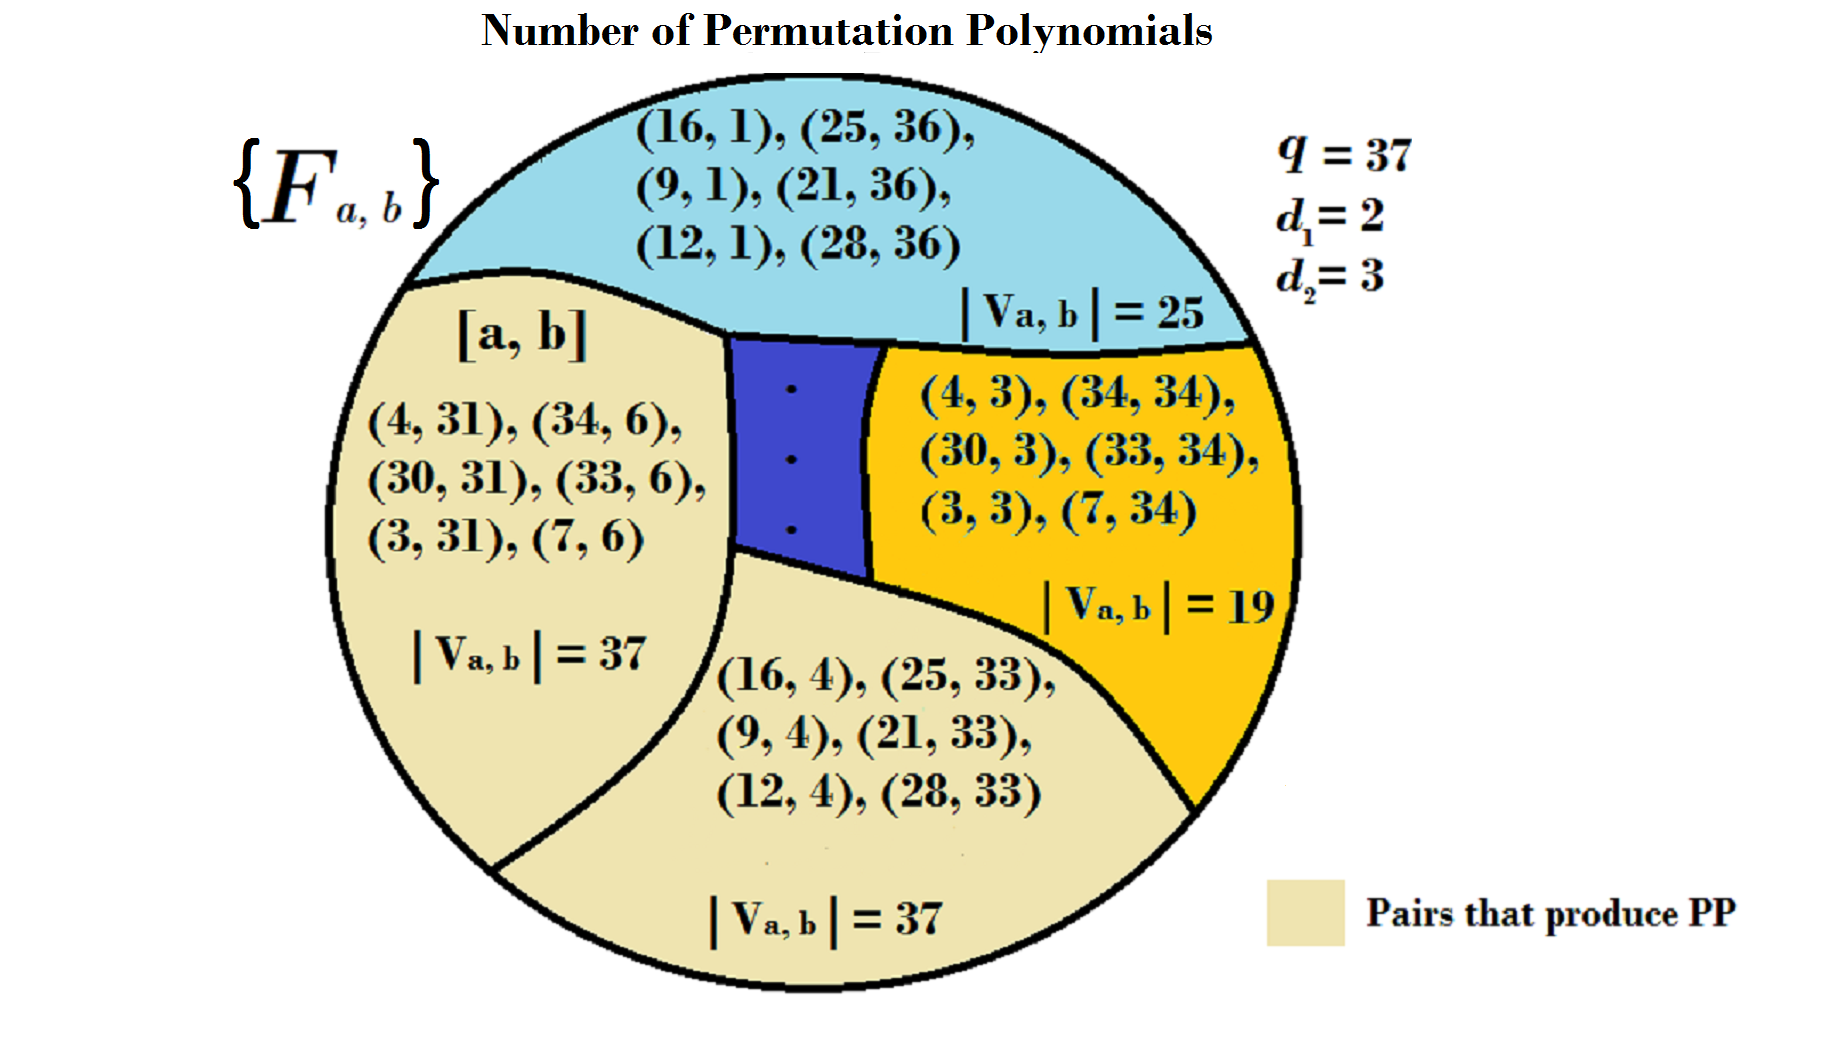
\includegraphics[width=11cm, height=6cm]{clases1}
\end{frame}

\begin{frame}{Value set correspondence}

  {\Large $$f_{a,b}(X) = X^r(X^{\frac{q-1}{d_1}} + aX^{\frac{q-1}{d_2}} +b)$$}

  $$$$

  \begin{theorem}

    Suppose that $f_{a, b} \sim f_{a',b'}$ then $|V(f_{a, b})| = |V(f_{a', b'})|$.

  \end{theorem}

  \begin{example}
    Let $q = 13, d_1 = 2, d_2 = 3, a = 4, b = 8$. Since $(2^2,2^3) \sim (2^4,2^9)$ we have that $|V(f_{2^2, 2^3})| = |V(f_{2^4, 2^9})| = 7$
  \end{example}

\end{frame}

\begin{frame}{Permutation Polynomial correspondence}

  {\Large $$f_{a,b}(X) = X^r(X^{\frac{q-1}{d_1}} + aX^{\frac{q-1}{d_2}} +b)$$}

  $$$$

  \begin{corollary}
    Suppose that $f_{a,b}$ is a permutation polynomial and $f_{a, b} \sim f_{a',b'}$, then $f_{a', b'}$ is also a permutation polynomial.
  \end{corollary}
\end{frame}

\begin{frame}{Size of equivalence classes}
  
  {\Large $$f_{a,b}(X) = X^r(X^{\frac{q-1}{d_1}} + aX^{\frac{q-1}{d_2}} +b)$$}

  $$$$

  \begin{proposition}
    $|[f_{a, b}]| = lcm(d_1,d_2)$ where $lcm(x,y)$ is the least common multiple of $x$ and $y$.
  \end{proposition}

  \begin{example}
    Let $q = 13, d_1 = 2, d_2 = 3, a = 4, b = 8$. Note that $lcm(2,3) = 6$ These are the elements of $(a,b)$:
    {\small $$\begin{array}{ccccccc}
                  (2^2, 2^3) & (2^4, 2^9) & (2^6, 2^3) & (2^8, 2^9) & (2^{10}, 2^3) & (2^{12}, 2^9) & (2^2, 2^3) \\
                  
                  (4, 8) & (3, 5) & (12, 8) & (9, 5) & (10, 8) & (1, 5) & (4, 8) 
                \end{array}$$}
  \end{example}
\end{frame}

\begin{frame}{Polynomials Results}
  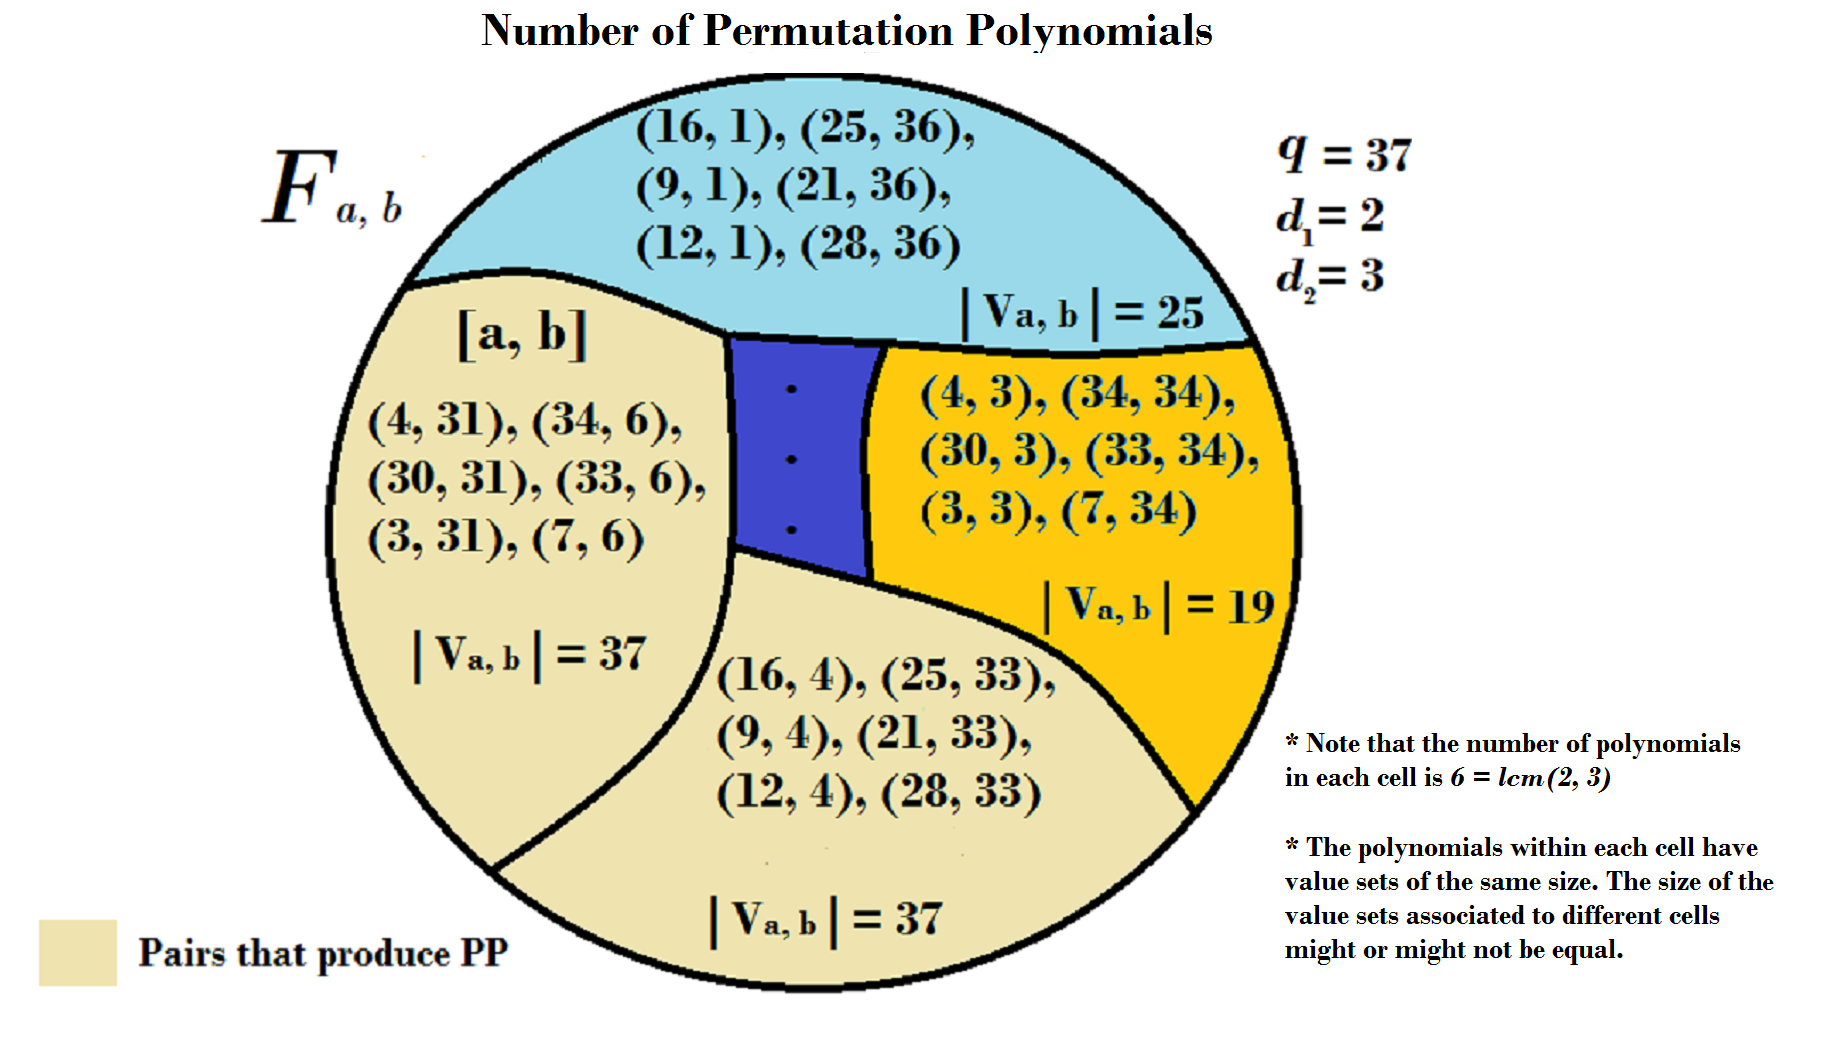
\includegraphics[width=11cm, height=6cm]{clases}
\end{frame}

\begin{frame}{Polynomial Results}
    \begin{proposition}
    The number of polynomials of the form $f_{a, b}(X)$ with $|V(f_{a, b})| = n$ is a multiple of $lcm(d_1, d_2)$
  \end{proposition}

  \begin{corollary}
    The number of permutation polynomials of the form $f_{a, b}(X)$ is a multiple of $lcm(d_1, d_2)$
  \end{corollary}
\end{frame}

% subsection families_of_polynomials_with_same_size_value_sets (end)

% \subsection{Construction of families of permutation trinomials} % (fold)
% \label{sub:construction_of_families_of_permutation_trinomials}

% \begin{frame}\frametitle{Constructing permutation trinomials}
    
% The following proposition gives us sufficient conditions for $f_{a,b}$ to be a permutation polynomial.

% \begin{proposition}
%   Suppose that $d\mid q-1$, $a, b \in \mathbb{F}_{q}$, $gcd(r, \frac{q^m-1}{r})=1$, and $h(X)=X^{\frac{d}{d_1}}+aX^{\frac{d}{d_2}}+b$. Let $gara = \alpha^{\frac{q-1}{d}}$, where $\alpha$ is a primitive root in $\mathbb{F}_{q}$. If $ (h(gara^i)/h(gara^j))^{\frac{q-1}{d}}=1 $ for all $0\leq i < j < d$, then $f_{a,b}(X)$ is a permutation polynomial of $\mathbb{F}_{q}$. 
% \end{proposition}

% \end{frame}

% subsection construction_of_families_of_permutation_trinomials (end)

\begin{frame}{Future Work}
  \begin{itemize}
    \item Find necessary and sufficient conditions such that $V(f_{a,b}) = \mathbb{F}_q$
    \vspace{0.8cm}
    \item Generalize results to polynomials with more terms and with exponents not divisors of $q-1$: $$f_{a,b}(X) = X^r(X^{d_1} + aX^{d_2} +b)$$
  \end{itemize}
\end{frame}

% section results (end)


\end{document}


